 %-------------------------------------------------------------------
% This is an outline file to help you with the writeup for Lab 1
% Edit this file
% To produce a typeset .pdf to submit, you need to do the following at 
% the command line:
% > pdflatex lab1sol
% This will produce a file lab1sol.pdf
%===================================================================

\documentclass[11pt, fleqn]{article}

%-------------------------------------------------------------------
%  - letter size may be 10, 11 or 12pt (I picked 11)
%    fleqn tells LaTeX that you want "flush left equations", default
%    will center the equations 
%===================================================================

\usepackage{amsfonts}

%-------------------------------------------------------------------
%  American Mathematical Society 
%  This package provides fonts useful for mathematics
%  You can see available symbols and their LaTeX control sequences at
%  http://amath.colorado.edu/documentation/LaTeX/Symbols.pdf
%===================================================================

\usepackage{graphicx}

%-------------------------------------------------------------------
%  This is so that I can later include graphic images into my document
%===================================================================


\topmargin=-1.5cm
\textheight=22cm
%-------------------------------------------------------------------
% Most things can be defaulted in LaTeX.  
% But you can change, for example, move the top margin up a little
%==================================================================

\title{CPS615 Winter 2015\\Lab 1 submission}
\author{Nikolas Maier, Std ID 500461990}
\date{\today}

\begin{document}
\maketitle
\section{Introduction and Overall Comments}
Hello, welcome to my lab report 

\section*{Solution to Exercise 1}

The language recognized by the automaton consists of the following set 
\[
\{w|w \mbox{ is a binary string and starts with 1 and ends with 0 }\}
\]

\section*{Solution to Exercise 2}

\subsection*{Part (1)}
The downloaded automaton does not recognize 
\[
\{w|w \mbox{ ends with a 1}\}
\]
as if the input is only a 1 then it will reject the string

\subsection*{Part (2)}
Automaton A 

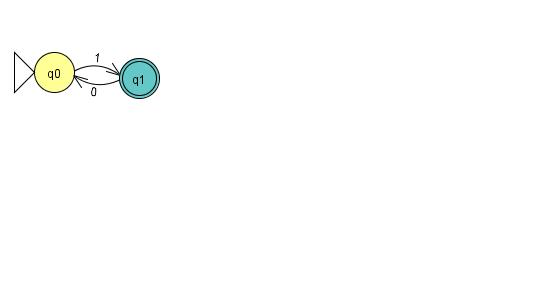
\includegraphics[scale=0.5]{https://github.com/Niktib/SchoolWork/blob/master/fa-a.jpg}

\pagebreak

Automaton B 

\includegraphics[scale=0.5]{https://github.com/Niktib/SchoolWork/blob/master/fa_b.jpg}

Automaton C

\includegraphics[scale=0.5]{https://github.com/Niktib/SchoolWork/blob/master/fa_c.jpg}

Automaton D

\includegraphics[scale=0.5]{https://github.com/Niktib/SchoolWork/blob/master/fa_d.jpg}

\pagebreak
Automaton E

\includegraphics[scale=0.5]{https://github.com/Niktib/SchoolWork/blob/master/fa_e.jpg}

\end{document}
